\documentclass[11pt,a4paper]{article}

% ---------- Packages ----------
\usepackage[T1]{fontenc}
\usepackage[utf8]{inputenc}
\usepackage[margin=2.5cm]{geometry}
\usepackage{graphicx}
\usepackage{xcolor}
\usepackage{tikz}
\usetikzlibrary{arrows.meta,positioning,shapes.geometric,fit,backgrounds,calc}
\usepackage{pgfplots}
\pgfplotsset{compat=1.18}
\usepackage{booktabs}
\usepackage{array}
\usepackage{longtable}
\usepackage{listings}
\usepackage{caption}
\usepackage{enumitem}
\usepackage{titlesec}
\usepackage{fancyhdr}
\usepackage{amssymb}
\usepackage{float}
\usepackage[hidelinks,colorlinks=true,linkcolor=NavyBlue,citecolor=NavyBlue,urlcolor=NavyBlue]{hyperref}

% ---------- Colors ----------
\definecolor{NavyBlue}{RGB}{0,51,102}
\definecolor{AgentBlue}{RGB}{209,229,255}
\definecolor{OrchOrange}{RGB}{255,224,178}
\definecolor{StoreGray}{RGB}{230,230,230}
\definecolor{CodeBg}{RGB}{245,245,245}
\definecolor{CodeKeyword}{RGB}{0,90,180}
\definecolor{CodeComment}{RGB}{110,110,110}
\definecolor{CodeString}{RGB}{160,40,40}

% ---------- Section styling ----------
\titleformat{\section}{\Large\bfseries\color{NavyBlue}}{\thesection}{0.5em}{}
\titleformat{\subsection}{\large\bfseries\color{NavyBlue!80!black}}{\thesubsection}{0.5em}{}

% ---------- Headers/footers ----------
\pagestyle{fancy}
\fancyhf{}
\fancyhead[L]{\small OpenEdu Orchestrator -- Implementation Report}
\fancyhead[R]{\small \thepage}
\renewcommand{\headrulewidth}{0.4pt}

% ---------- Code listing styles ----------
\lstdefinestyle{pystyle}{
    backgroundcolor=\color{CodeBg},
    basicstyle=\ttfamily\footnotesize,
    keywordstyle=\color{CodeKeyword}\bfseries,
    commentstyle=\color{CodeComment}\itshape,
    stringstyle=\color{CodeString},
    numbers=left,
    numberstyle=\tiny\color{gray},
    numbersep=8pt,
    frame=single,
    rulecolor=\color{gray!50},
    breaklines=true,
    showstringspaces=false,
    tabsize=4,
    language=Python,
    xleftmargin=1.2em,
}

\lstdefinestyle{termstyle}{
    backgroundcolor=\color{black!92},
    basicstyle=\ttfamily\footnotesize\color{white},
    frame=single,
    rulecolor=\color{gray!50},
    breaklines=true,
    showstringspaces=false,
    xleftmargin=1.2em,
}

\lstset{style=pystyle}

\newcommand{\ttu}[1]{\texttt{\detokenize{#1}}}

% ---------- Title page info ----------
\title{
    \vspace{-2cm}
    {\Huge \bfseries \color{NavyBlue} OpenEdu Orchestrator}\\[0.4cm]
    {\Large An Agentic Multi-Agent Data Synchronization System}\\[0.2cm]
    {\large PIEAS Website $\rightarrow$ OpenEduCat (Odoo) ERP}\\[0.3cm]
    {\normalsize \itshape Implementation Report -- Test Build on Dummy Data}
}
\author{Muhammad Shayan Asif}
\date{\today}

% ---------- TikZ reusable styles ----------
\tikzset{
    comp/.style={draw, thick, rounded corners, fill=StoreGray, minimum width=3.3cm, minimum height=1.05cm, align=center, font=\small},
    agentbox/.style={draw, thick, rounded corners, fill=AgentBlue, minimum width=3.3cm, minimum height=1.05cm, align=center, font=\small},
    orchbox/.style={draw, thick, rounded corners, fill=OrchOrange, minimum width=3.6cm, minimum height=1.2cm, align=center, font=\small},
    solidarr/.style={-{Latex[length=2.5mm]}, thick},
    dashedarr/.style={-{Latex[length=2.5mm]}, thick, dashed, gray!60!black},
    term/.style={draw, thick, circle, fill=gray!15, minimum size=0.95cm, font=\small},
    stage/.style={draw, thick, rounded corners, fill=AgentBlue, minimum width=4.0cm, minimum height=0.9cm, align=center, font=\small},
}

\begin{document}

\begin{titlepage}
\maketitle
\thispagestyle{empty}
\vspace{1cm}
\begin{center}
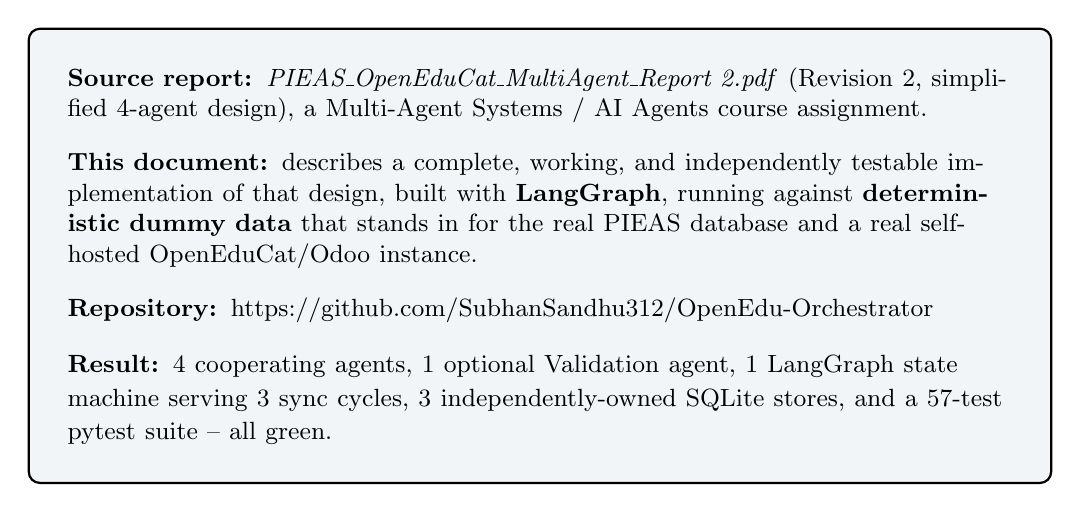
\begin{tikzpicture}
\node[draw, thick, rounded corners, fill=NavyBlue!5, align=left, text width=12cm, inner sep=14pt] (box) {
    \small
    \textbf{Source report:} \textit{PIEAS\_OpenEduCat\_MultiAgent\_Report 2.pdf} (Revision~2, simplified 4-agent design), a Multi-Agent Systems / AI Agents course assignment.\\[0.3cm]
    \textbf{This document:} describes a complete, working, and independently testable implementation of that design, built with \textbf{LangGraph}, running against \textbf{deterministic dummy data} that stands in for the real PIEAS database and a real self-hosted OpenEduCat/Odoo instance.\\[0.3cm]
    \textbf{Repository:} \url{https://github.com/SubhanSandhu312/OpenEdu-Orchestrator}\\[0.3cm]
    \textbf{Result:} 4 cooperating agents, 1 optional Validation agent, 1 LangGraph state machine serving 3 sync cycles, 3 independently-owned SQLite stores, and a 57-test pytest suite -- all green.
};
\end{tikzpicture}
\end{center}
\vfill
\end{titlepage}

\tableofcontents
\newpage

% =========================================================================
\section{Executive Summary}
% =========================================================================

This project turns a course-assignment design document into working software. The source
report specifies an \textbf{agentic, multi-agent system} for moving data one time from the
PIEAS website into OpenEduCat (an Odoo-based Student Information System), and then keeping the
two in sync forever after -- despite PIEAS exposing no API and no webhooks of any kind.

The implementation delivered here is not a diagram-only or pseudocode exercise. It is a
runnable Python package that:

\begin{itemize}[leftmargin=1.4em]
    \item implements all four agents the report specifies (\textbf{Extractor}, \textbf{Transformer},
          \textbf{Loader}, \textbf{Orchestrator}) plus the optional fifth \textbf{Validation Agent},
          with the exact non-overlapping responsibilities the report defines;
    \item wires them together as a single \textbf{LangGraph} \texttt{StateGraph} that serves all
          three operating cycles the report describes: bulk migration, the timestamp-watermark
          change cycle, and the full-ID-list deletion cycle;
    \item runs against a \textbf{deterministic dummy PIEAS database} (60 students, 18 faculty,
          14 courses, generated with a fixed random seed) and a \textbf{mock OpenEduCat/Odoo
          client} that exposes the same method surface (\texttt{create}, \texttt{write},
          \texttt{search\_read}, \texttt{read}) that a real Odoo XML-RPC connection would;
    \item enforces the report's strict agent-ownership rules \emph{structurally}, by giving each
          agent module a connection to exactly one of three separate SQLite databases;
    \item is verified by a \textbf{57-test pytest suite} covering every agent in isolation, every
          cycle end-to-end (including pagination and idempotency), and a full cross-entity
          lifecycle scenario; and
    \item ships a \textbf{command-line interface} (\texttt{seed}, \texttt{migrate}, \texttt{sync},
          \texttt{deletion-check}, \texttt{mutate}, \texttt{status}, \texttt{demo}) that lets
          anyone watch the whole design work end to end with a single command.
\end{itemize}

% =========================================================================
\section{Background and Problem Statement}
% =========================================================================

\subsection{Why this system exists}

PIEAS currently maintains its own website/system holding student, faculty, and course data.
The institution wants to adopt \textbf{OpenEduCat} -- a free, open-source, LGPL-3 Student
Information System built as a set of modules on top of \textbf{Odoo} -- as its system of record
going forward. Odoo is a modular ERP with a Python backend and a PostgreSQL database whose
Object-Relational Mapping (ORM) layer enforces validation, computed fields, and related-record
bookkeeping on every write; bypassing it (writing straight to PostgreSQL) risks silent,
half-formed data with no error raised.

This creates two distinct problems, both of which the source report frames as requiring an
\emph{agentic} solution rather than a single script:

\begin{enumerate}[leftmargin=1.4em]
    \item \textbf{One-time migration} -- every existing PIEAS record must be transferred into
          OpenEduCat before it can become the system of record.
    \item \textbf{Ongoing synchronization} -- after migration, PIEAS keeps being used. New
          students are admitted, records are edited, and some are removed. OpenEduCat must
          reflect all of this automatically.
\end{enumerate}

\subsection{The constraint that shapes everything}

\begin{quote}
\itshape
``PIEAS exposes no API and no webhooks. It cannot notify anything when its data changes. Any
detection of change, and any detection of deletion, has to happen by actively checking PIEAS,
not by PIEAS pushing updates out.''
\end{quote}

This single constraint is why the system needs a scheduler-driven, stateful comparison loop
(the Orchestrator) rather than an event-driven integration -- and why detecting a
\emph{deletion} turns out to require an entirely different query shape than detecting a
\emph{change} (Section~\ref{sec:change-deletion}).

% =========================================================================
\section{System Architecture}
% =========================================================================

\subsection{Design principle: one agent, one clear job}

The report considered, and deliberately rejected, a fifth ``Monitor'' agent dedicated to change
detection -- its job (deciding when to check PIEAS, comparing results against known state)
overlapped entirely with the Orchestrator's, since the Orchestrator already owns the state
needed to do that comparison. The final design therefore has four agents with strictly
non-overlapping responsibilities:

\begin{itemize}[leftmargin=1.4em]
    \item \textbf{Only the Extractor} ever talks to PIEAS. It is a pure fetcher with no memory
          between calls and no opinion about what the data means.
    \item \textbf{Only the Orchestrator} makes decisions. It is the only agent that reads or
          writes the local state store.
    \item \textbf{Transformer and Loader are stateless workers.} Each does exactly one job on
          whatever it is handed, regardless of which cycle triggered it.
\end{itemize}

\subsection{Architecture diagram}

\begin{figure}[H]
\centering
\resizebox{\textwidth}{!}{%
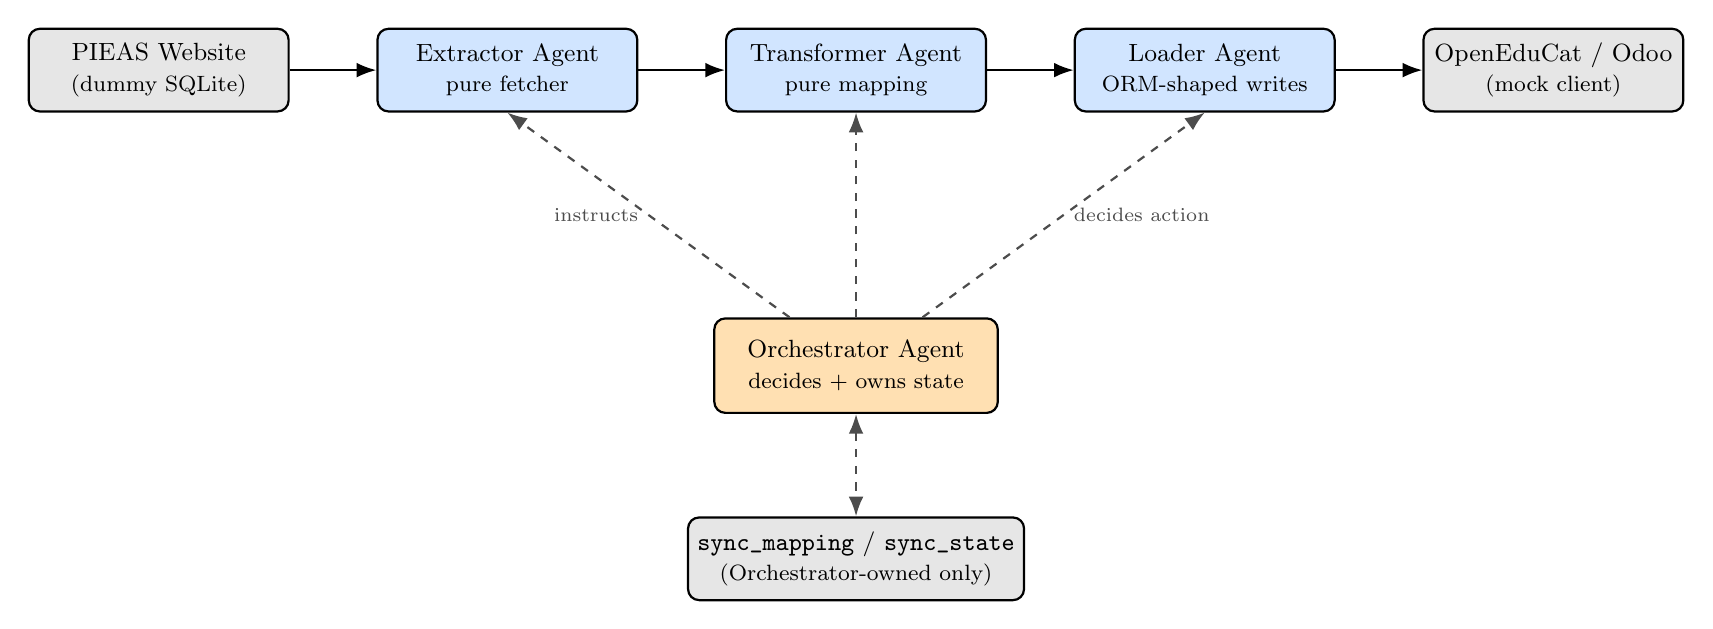
\begin{tikzpicture}[node distance=1.0cm and 1.1cm]
\node[comp] (pieas) {PIEAS Website\\\footnotesize (dummy SQLite)};
\node[agentbox, right=of pieas] (extractor) {Extractor Agent\\\footnotesize pure fetcher};
\node[agentbox, right=of extractor] (transformer) {Transformer Agent\\\footnotesize pure mapping};
\node[agentbox, right=of transformer] (loader) {Loader Agent\\\footnotesize ORM-shaped writes};
\node[comp, right=of loader] (oc) {OpenEduCat / Odoo\\\footnotesize (mock client)};

\node[orchbox, below=2.6cm of transformer] (orch) {Orchestrator Agent\\\footnotesize decides + owns state};
\node[comp, below=1.3cm of orch] (state) {\ttu{sync_mapping} / \ttu{sync_state}\\\footnotesize (Orchestrator-owned only)};

\draw[solidarr] (pieas) -- (extractor);
\draw[solidarr] (extractor) -- (transformer);
\draw[solidarr] (transformer) -- (loader);
\draw[solidarr] (loader) -- (oc);

\draw[dashedarr] (orch) -- (extractor.south) node[midway, left, font=\scriptsize] {instructs};
\draw[dashedarr] (orch) -- (transformer.south);
\draw[dashedarr] (orch) -- (loader.south) node[midway, right, font=\scriptsize] {decides action};
\draw[dashedarr, {Latex[length=2.5mm]}-{Latex[length=2.5mm]}] (orch) -- (state);
\end{tikzpicture}%
}
\caption{Four-agent architecture. Solid arrows are the data pipeline (PIEAS $\rightarrow$
OpenEduCat); dashed arrows are instructions and state ownership, all controlled by the
Orchestrator -- the only agent with memory of prior syncs.}
\label{fig:architecture}
\end{figure}

\subsection{Three independently-owned databases}

The separation of concerns above is enforced \emph{structurally}, not just by convention: three
separate SQLite files stand in for three separate real systems, and only one agent module has a
code path to open each one.

\begin{table}[H]
\centering
\small
\begin{tabular}{@{}p{5.3cm}p{4.0cm}p{4.4cm}@{}}
\toprule
\textbf{Database file} & \textbf{Stands in for} & \textbf{Only opened by} \\
\midrule
\ttu{data/pieas.db} & The PIEAS website's database & \texttt{ExtractorAgent} \\[0.3em]
\ttu{data/openeducat_mock.db} & Self-hosted Odoo + OpenEduCat & \texttt{LoaderAgent} (writes), \texttt{ValidationAgent} (reads) \\[0.3em]
\ttu{data/orchestrator_state.db} & N/A -- exists only for this system & \texttt{OrchestratorAgent} \\
\bottomrule
\end{tabular}
\caption{Database ownership boundaries.}
\end{table}

% =========================================================================
\section{Agent-by-Agent Breakdown}
% =========================================================================

\begin{table}[H]
\centering
\small
\begin{tabular}{@{}p{2.3cm}p{9.0cm}p{2.9cm}@{}}
\toprule
\textbf{Agent} & \textbf{Responsibility} & \textbf{Module} \\
\midrule
Extractor & Pure fetcher; the only agent that ever contacts PIEAS. Dispatches on an
instruction: \ttu{fetch_changed} (watermarked rows), \ttu{fetch_page} (paginated full pull),
or \ttu{fetch_ids} (bare ID list for deletion detection). Holds no state between calls. &
\texttt{extractor.py} \\[0.4em]
Transformer & Maps a PIEAS-shaped record onto an OpenEduCat-shaped record, per entity type
(\texttt{op.student}, \texttt{op.faculty}, \texttt{op.course}). A pure function: identical
input always produces identical output, with no I/O and no awareness of create vs.\ update. &
\texttt{transformer.py} \\[0.4em]
Loader & Writes into OpenEduCat via an ORM-shaped client. Executes exactly the action it is
told: \texttt{create}, \texttt{update} (write), or \texttt{archive} (write \texttt{active=False}).
Makes no decisions of its own. & \texttt{loader.py} \\[0.4em]
Orchestrator & The only decision-making agent. Owns and is the sole reader/writer of
\ttu{sync_mapping} and \ttu{sync_state}. Decides what to fetch, classifies every record as
\texttt{create}/\texttt{update}/\texttt{unchanged}, and (in the deletion cycle)
\texttt{archive}. Owns the switch from BULK mode to SYNC mode. & \texttt{orchestrator.py} \\[0.4em]
Validator \textit{(optional)} & Re-reads a record after a Loader write and confirms it matches
what was sent. Purely observational -- never blocks or retries a write itself; findings are
advisory and appended to the run report. & \texttt{validator.py} \\
\bottomrule
\end{tabular}
\caption{Agent responsibilities, mirroring the source report's Section 3.3 / 3.4 exactly.}
\end{table}

\subsection{Illustrative excerpt: the Orchestrator's classification logic}

This is the heart of the decision-making agent -- the code that decides \texttt{create} vs.\
\texttt{update} vs.\ \texttt{unchanged} for every fetched PIEAS row, by looking up the mapping
table and comparing a content hash:

\begin{lstlisting}[caption={Orchestrator record classification (\texttt{agents/orchestrator.py}).}]
def classify_records(self, entity_type, records):
    classified = []
    for record in records:
        pieas_id = record["pieas_id"]
        business_fields = {k: v for k, v in record.items() if k != "last_updated"}
        h = store.content_hash(business_fields)
        mapping = store.get_mapping(self._conn, pieas_id, entity_type)
        if mapping is None:
            action, openeducat_id = "create", None
        elif mapping["content_hash"] == h:
            action, openeducat_id = "unchanged", mapping["openeducat_id"]
        else:
            action, openeducat_id = "update", mapping["openeducat_id"]
        classified.append({
            "entity_type": entity_type, "pieas_id": pieas_id, "action": action,
            "source_record": record, "openeducat_id": openeducat_id, "content_hash": h,
        })
    return classified
\end{lstlisting}

% =========================================================================
\section{The LangGraph Orchestration Layer}
% =========================================================================

\subsection{Why one graph, not three}

Bulk migration, the change cycle, and the deletion cycle all share the same
Extractor~$\rightarrow$~Transformer~$\rightarrow$~Loader pipeline; they differ only in what the
Orchestrator asks the Extractor to fetch and what it does with the result. Rather than building
three separate LangGraph graphs, the implementation builds \textbf{one} \texttt{StateGraph}
whose nodes branch on a \texttt{mode} field (\texttt{"bulk"}, \texttt{"change"}, or
\texttt{"deletion"}) carried in the graph state. This keeps the report's cycles honest about
sharing a pipeline, instead of accidentally re-implementing three near-identical graphs.

\subsection{Pipeline state machine}

\begin{figure}[H]
\centering
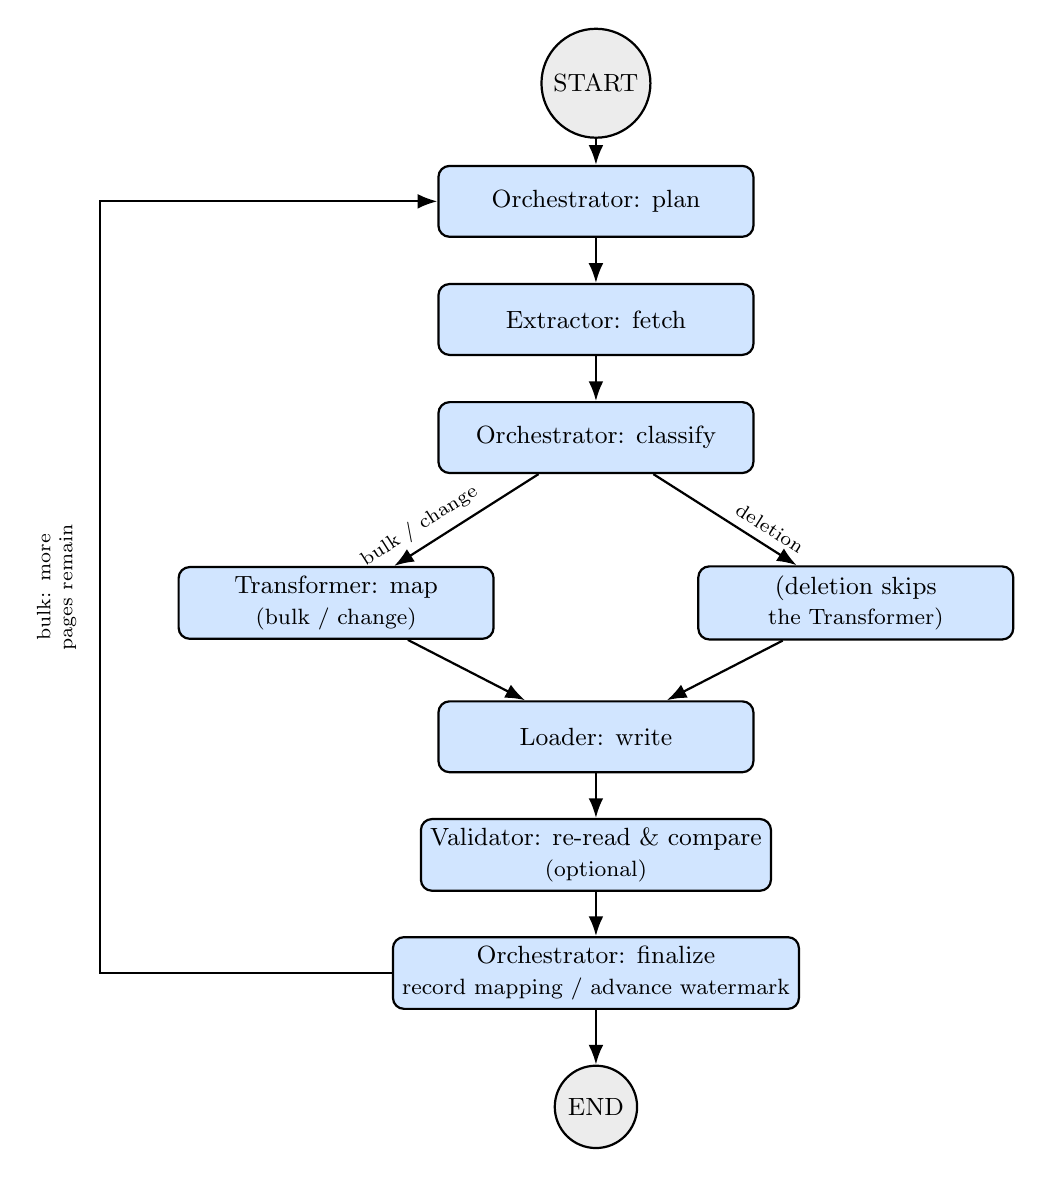
\begin{tikzpicture}
\node[term] (start) at (0,13.2) {START};
\node[stage] (plan) at (0,11.7) {Orchestrator: plan};
\node[stage] (extract) at (0,10.2) {Extractor: fetch};
\node[stage] (classify) at (0,8.7) {Orchestrator: classify};
\node[stage] (transform) at (-3.3,6.6) {Transformer: map\\\footnotesize (bulk / change)};
\node[stage] (skip) at (3.3,6.6) {(deletion skips\\\footnotesize the Transformer)};
\node[stage] (load) at (0,4.9) {Loader: write};
\node[stage] (validate) at (0,3.4) {Validator: re-read \& compare\\\footnotesize (optional)};
\node[stage] (finalize) at (0,1.9) {Orchestrator: finalize\\\footnotesize record mapping / advance watermark};
\node[term] (end) at (0,0.2) {END};

\draw[solidarr] (start) -- (plan);
\draw[solidarr] (plan) -- (extract);
\draw[solidarr] (extract) -- (classify);
\draw[solidarr] (classify) -- node[pos=0.75, above, sloped, font=\scriptsize] {bulk / change} (transform);
\draw[solidarr] (classify) -- node[pos=0.75, above, sloped, font=\scriptsize] {deletion} (skip);
\draw[solidarr] (transform) -- (load);
\draw[solidarr] (skip) -- (load);
\draw[solidarr] (load) -- (validate);
\draw[solidarr] (validate) -- (finalize);
\draw[solidarr] (finalize) -- (end);
\coordinate (loopbottom) at (-6.3,1.9);
\coordinate (looptop) at (-6.3,11.7);
\draw[solidarr] (finalize.west) -- (loopbottom) -- (looptop) -- (plan.west);
\node[font=\scriptsize, align=center, text width=2.4cm, rotate=90] at ($(loopbottom)!0.5!(looptop)+(-0.55,0)$) {bulk: more pages remain};
\end{tikzpicture}
\caption{The shared LangGraph \texttt{StateGraph}. \texttt{mode} decides branching at
\textit{classify} (whether the Transformer is invoked) and at \textit{finalize} (whether bulk
migration loops back for another page or the run ends).}
\label{fig:pipeline}
\end{figure}

\subsection{A subtlety worth documenting: pagination and running totals}

LangGraph state keys are last-write-wins by default (no reducer was declared for the count
fields). Bulk migration loops \textit{plan}~$\rightarrow$~\textit{finalize} once per page, so a
naive implementation that read \texttt{classified}/\texttt{load\_results} directly from the
\emph{final} graph state after the whole run would only see the \textbf{last page's} numbers --
silently under-reporting a multi-page bulk migration's totals. This was caught during
integration testing (Section~\ref{sec:testing}) and fixed by carrying running totals
(\texttt{total\_fetched}, \texttt{total\_created}, \dots) inside the state itself, with each
pass through \textit{finalize} adding that page's counts onto the total already carried
forward:

\begin{lstlisting}[caption={Running-total accumulation across bulk-migration pages (\texttt{graph.py}).}]
update = {
    "total_fetched": state.get("total_fetched", 0) + page_fetched,
    "total_created": state.get("total_created", 0) + page_created,
    "total_updated": state.get("total_updated", 0) + page_updated,
    "total_unchanged": state.get("total_unchanged", 0) + page_unchanged,
    "total_archived": state.get("total_archived", 0) + page_archived,
}
if state["mode"] == "bulk" and state.get("more_pages"):
    update["page_offset"] = state.get("page_offset", 0) + state.get("page_size", BULK_PAGE_SIZE)
return update
\end{lstlisting}

% =========================================================================
\section{Change Detection and Deletion Detection}
\label{sec:change-deletion}
% =========================================================================

\subsection{Change detection: timestamp watermark}

The report considered and rejected a boolean ``dirty flag'' column reset after each sync, on
the grounds that resetting it blindly can silently drop a second change that arrives while a
row is mid-sync (a race condition). The adopted method instead keeps a
\ttu{last_updated} timestamp per row and a single \ttu{last_synced_at} watermark the
Orchestrator owns:

\begin{lstlisting}[language=SQL,caption={Change-cycle query (adapted per entity table).}]
SELECT * FROM students
WHERE last_updated > :watermark
ORDER BY last_updated ASC;
\end{lstlisting}

This implementation adds one refinement beyond the report's literal text: the watermark
advances to the \textbf{maximum \ttu{last_updated} actually processed in the run}, not to
wall-clock \texttt{NOW()}. This is safer against a row changing again while a run is in
progress than the report's literal \texttt{UPDATE sync\_state SET last\_synced\_at = NOW()}.

\subsection{Deletion detection: full ID list, compared locally}

A filtered \ttu{last_updated} query can never see a deletion -- a row that no longer exists is
simply never returned. Detecting a deletion therefore requires a structurally different,
less-frequent check:

\begin{enumerate}[leftmargin=1.4em]
    \item The Extractor fetches the \textbf{full, unfiltered} list of PIEAS IDs (IDs only, to
          keep the pull cheap).
    \item The Orchestrator compares that list against its own \ttu{sync_mapping} table --
          \textbf{locally}; PIEAS is not queried again. Any mapping row whose \texttt{pieas\_id}
          is absent from the fetched list is a detected deletion.
\end{enumerate}

The report expresses this comparison as a \texttt{LEFT JOIN ... WHERE ... IS NULL} against a
live database table. Because \ttu{sync_mapping} and the PIEAS table live in genuinely separate
SQLite files in this build, the equivalent comparison is done as a Python set difference over
the two locally-available lists -- semantically identical to the report's \texttt{LEFT JOIN},
without requiring a fragile cross-database \texttt{ATTACH}.

\subsection{What happens to a detected deletion}

Per the report's Section 5.4, the adopted handling is to \textbf{archive}, not hard-delete: the
Loader issues \texttt{write(model, id, \{"active": False\})}. The record disappears from normal
OpenEduCat views but its history (grades, past enrollment) is preserved, and the action is
reversible if a ``deletion'' on PIEAS was actually a rename.

\subsubsection*{A known, intentional characteristic}

Once a record is permanently gone from PIEAS, \emph{every} subsequent deletion cycle will still
find its mapping row and re-issue the archive write, since nothing in the report's schema marks
a mapping as ``already handled.'' This is harmless -- archiving an already-inactive record is a
no-op against real Odoo too -- but it does mean the deletion cycle's reported \texttt{archived}
count means ``archive calls issued,'' not strictly ``newly discovered deletions.'' This was a
deliberate choice to avoid inventing a field the source report does not specify.

% =========================================================================
\section{Database Schemas}
% =========================================================================

\begin{table}[H]
\centering
\small
\begin{tabular}{@{}p{2.0cm}p{9.4cm}p{1.6cm}@{}}
\toprule
\textbf{Table} & \textbf{Key columns} & \textbf{Entity} \\
\midrule
\texttt{students} & pieas\_id (PK), roll\_number, first/last\_name, email, gender,
date\_of\_birth, department, batch\_year, last\_updated & student \\
\texttt{faculty} & pieas\_id (PK), employee\_code, first/last\_name, email, department,
designation, last\_updated & faculty \\
\texttt{courses} & pieas\_id (PK), code, name, department, credit\_hours, semester,
last\_updated & course \\
\bottomrule
\end{tabular}
\caption{Dummy PIEAS schema. A trigger on each table bumps \texttt{last\_updated} automatically
whenever an \texttt{UPDATE} does not set it explicitly, exactly mirroring how a real database's
auto-maintained timestamp column behaves.}
\end{table}

\begin{table}[H]
\centering
\small
\begin{tabular}{@{}p{2.0cm}p{8.8cm}p{2.2cm}@{}}
\toprule
\textbf{Table} & \textbf{Key columns} & \textbf{Odoo model} \\
\midrule
\texttt{op\_student} & id (PK), pieas\_id, name, email, gender, birth\_date, department,
batch\_year, active, create/write\_date & \texttt{op.student} \\
\texttt{op\_faculty} & id (PK), pieas\_id, name, email, department, designation, active,
create/write\_date & \texttt{op.faculty} \\
\texttt{op\_course} & id (PK), pieas\_id, code, name, department, credit\_hours, semester,
active, create/write\_date & \texttt{op.course} \\
\bottomrule
\end{tabular}
\caption{Mock OpenEduCat schema -- deliberately mirrors real Odoo conventions (\texttt{active},
\texttt{write\_date}).}
\end{table}

\begin{table}[H]
\centering
\small
\begin{tabular}{@{}lp{9.6cm}@{}}
\toprule
\textbf{Table (Orchestrator-owned)} & \textbf{Columns} \\
\midrule
\ttu{sync_mapping} & id (PK), pieas\_id, openeducat\_id, entity\_type, content\_hash,
last\_synced\_at -- \texttt{UNIQUE(pieas\_id, entity\_type)} \\
\ttu{sync_state} & entity\_type (PK), last\_synced\_at \\
\bottomrule
\end{tabular}
\caption{Orchestrator's private state store -- taken directly from the report's Listing 4, with
\texttt{content\_hash} used as a bonus refinement (Section~\ref{sec:refinements}).}
\end{table}

% =========================================================================
\section{Design Decisions Carried Over From the Report}
% =========================================================================

\begin{table}[H]
\centering
\small
\begin{tabular}{@{}p{4.6cm}p{9.4cm}@{}}
\toprule
\textbf{Decision point} & \textbf{Resolution (as implemented)} \\
\midrule
Change detection mechanism & Timestamp watermark, not a boolean dirty flag -- avoids the
reset race condition. \\
Deletion detection mechanism & Separate, less-frequent cycle: full ID fetch, compared locally
against \ttu{sync_mapping}. \\
What to do with a detected deletion & Archive (\texttt{active=False}), not hard-delete --
reversible, preserves history. \\
How to write into the target & Through an ORM-shaped interface (\texttt{create}/\texttt{write}),
never raw SQL -- preserves validation and computed-field behaviour. \\
Was a separate Monitor Agent needed? & No -- its responsibilities are absorbed by the
Orchestrator, which already owns the state needed for the comparison. \\
\bottomrule
\end{tabular}
\caption{Every major design fork in the source report, and how this implementation resolves it
-- unchanged from the report's own conclusions.}
\end{table}

\section{Refinements Beyond the Report's Literal Text}
\label{sec:refinements}

Two small engineering decisions go slightly beyond what the report specifies verbatim, both
documented in code comments and in the project's \texttt{README.md} so they are never mistaken
for the report's own design:

\begin{enumerate}[leftmargin=1.4em]
    \item \textbf{Watermark advances by processed maximum, not \texttt{NOW()}.} Safer against a
          row changing again mid-run than the report's literal Listing~7.
    \item \textbf{A content-hash check layered on top of the watermark.} A record whose
          \texttt{last\_updated} was touched but whose business fields are byte-for-byte
          identical classifies as \texttt{unchanged} rather than \texttt{update}. This also lets
          \textbf{bulk migration seed the watermark itself}, so the very first change cycle
          afterwards does not have to re-fetch and re-classify every just-migrated row only to
          discover where the watermark should start.
\end{enumerate}

% =========================================================================
\section{Technology Stack}
% =========================================================================

\begin{table}[H]
\centering
\small
\begin{tabular}{@{}p{2.1cm}p{3.3cm}p{7.6cm}@{}}
\toprule
\textbf{Library} & \textbf{Role} & \textbf{Why} \\
\midrule
\texttt{langgraph} & Orchestration graph / state machine & Purpose-built for exactly this kind
of stateful, branching agent pipeline; not restricted to LLM-driven agents. \\
\texttt{pydantic} & Typed data models & Malformed records fail loudly at a model boundary
instead of silently corrupting a write. \\
\texttt{sqlite3} (stdlib) & Three data stores & Zero external services needed to run or test the
whole system; trivially swappable for a real driver later. \\
\texttt{Faker} & Deterministic dummy data & Reproducible fake PIEAS records with a fixed seed. \\
\texttt{click} & CLI & Clean subcommands (\texttt{seed}, \texttt{migrate}, \texttt{sync}, ...). \\
\texttt{rich} & CLI output formatting & Readable tables/console output for the \texttt{status}
and \texttt{demo} commands. \\
\texttt{pytest} & Test suite & 57 tests, fixtures for isolated per-test databases via
\texttt{tmp\_path}. \\
\bottomrule
\end{tabular}
\caption{Full dependency list (\texttt{requirements.txt}).}
\end{table}

\textbf{Note on ``agentic'':} no LLM calls are made anywhere in this pipeline. The system is
agentic in the report's own sense -- autonomous, cooperating components with clearly separated
responsibilities and a decision-making Orchestrator -- implemented deterministically so that
every run is reproducible and testable byte-for-byte. LangGraph was chosen specifically because
it models this kind of stateful multi-step orchestration regardless of whether any step calls
an LLM; nothing about the design would change if a future extension (e.g., an LLM-assisted
Transformer for messy/ambiguous field mapping) were added on top.

% =========================================================================
\section{Testing and Quality Assurance}
\label{sec:testing}
% =========================================================================

\subsection{Suite structure}

\begin{figure}[H]
\centering
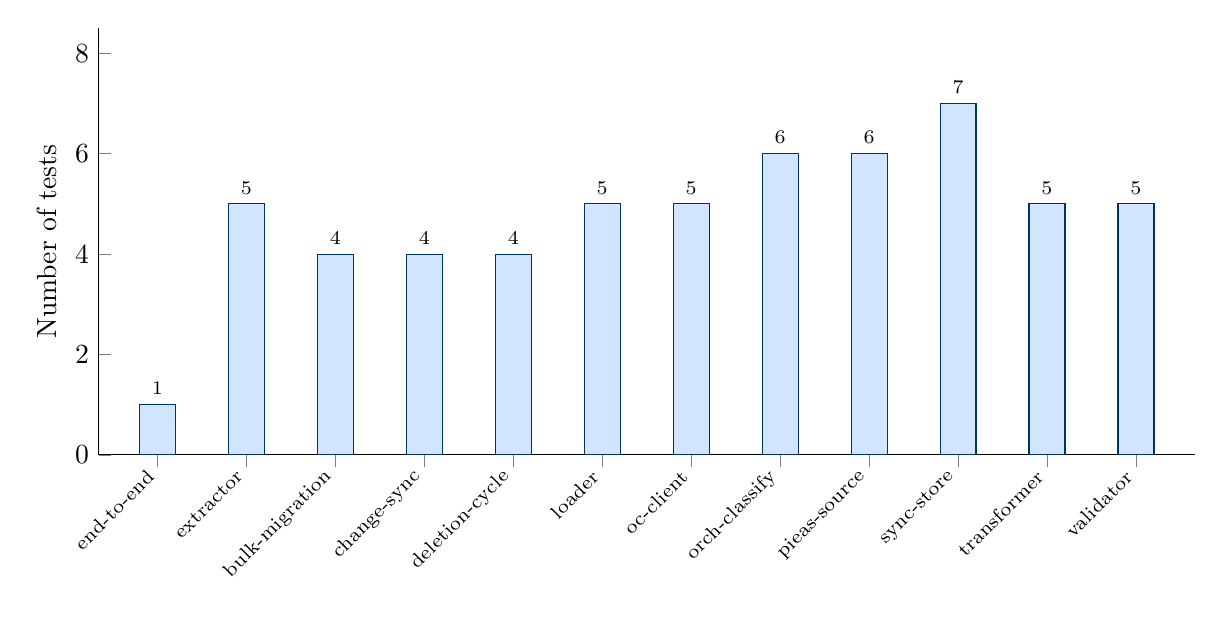
\begin{tikzpicture}
\begin{axis}[
    ybar,
    bar width=13pt,
    width=15.5cm, height=7cm,
    symbolic x coords={end-to-end,extractor,bulk-migration,change-sync,deletion-cycle,
                        loader,oc-client,orch-classify,pieas-source,sync-store,transformer,validator},
    xtick=data,
    x tick label style={rotate=45, anchor=east, font=\scriptsize},
    ylabel={Number of tests},
    ymin=0, ymax=8.5,
    nodes near coords,
    every node near coord/.append style={font=\scriptsize},
    enlarge x limits=0.06,
    axis lines*=left,
    ]
\addplot[fill=AgentBlue, draw=NavyBlue] coordinates {
    (end-to-end,1) (extractor,5) (bulk-migration,4) (change-sync,4) (deletion-cycle,4)
    (loader,5) (oc-client,5) (orch-classify,6) (pieas-source,6)
    (sync-store,7) (transformer,5) (validator,5)
};
\end{axis}
\end{tikzpicture}
\caption{Distribution of the 57-test pytest suite across test modules.}
\label{fig:testchart}
\end{figure}

\begin{table}[H]
\centering
\small
\begin{tabular}{@{}p{6.9cm}p{7.0cm}@{}}
\toprule
\textbf{Test file} & \textbf{What it verifies} \\
\midrule
\texttt{test\_pieas\_source.py} & Schema, seeding, pagination, watermark filtering, trigger-based
timestamp bump, real row deletion. \\
\texttt{test\_openeducat\_client.py} & \texttt{create}/\texttt{write}/\texttt{archive}, domain
filtering, unknown-model error handling. \\
\texttt{test\_sync\_store.py} & Upsert semantics, per-entity scoping, watermark read/write,
content-hash stability. \\
\texttt{test\_extractor.py} & Instruction dispatch, statelessness across calls. \\
\texttt{test\_transformer.py} & Per-entity field mapping, purity, unknown-entity error. \\
\texttt{test\_loader.py} & Create/update/archive execution, graceful failure on a bad update. \\
\texttt{test\_orchestrator\_classification.py} & create/update/unchanged classification,
deletion-candidate detection, per-entity scoping, bulk-mode flip. \\
\texttt{test\_validator.py} & Field-match and mismatch detection, archive-state verification. \\
\texttt{test\_graph\_bulk\_migration.py} & Multi-page pagination totals, per-entity isolation,
re-run idempotency. \\
\texttt{test\_graph\_change\_sync.py} & Edit + new-admission detection, no-op reruns, watermark
monotonicity, cross-entity isolation. \\
\texttt{test\_graph\_deletion\_cycle.py} & Archival correctness, and the structural proof that
the change cycle \textit{cannot} see a deletion. \\
\texttt{test\_end\_to\_end.py} & Full lifecycle across all three entity types in one scenario. \\
\bottomrule
\end{tabular}
\caption{Test file responsibilities.}
\end{table}

\subsection{Test run output}

\begin{lstlisting}[style=termstyle,caption={Actual output of the full suite.}]
$ python -m pytest -v
============================= test session starts =============================
collected 57 items

tests/test_end_to_end.py::test_full_lifecycle_across_all_entity_types    PASSED
tests/test_extractor.py ......................................... 5 passed
tests/test_graph_bulk_migration.py ......................... 4 passed
tests/test_graph_change_sync.py ............................ 4 passed
tests/test_graph_deletion_cycle.py ......................... 4 passed
tests/test_loader.py ....................................... 5 passed
tests/test_openeducat_client.py ............................ 5 passed
tests/test_orchestrator_classification.py .................. 6 passed
tests/test_pieas_source.py ................................. 6 passed
tests/test_sync_store.py .................................... 7 passed
tests/test_transformer.py .......................... 5 passed
tests/test_validator.py .............................. 5 passed

============================= 57 passed in 2.93s ===============================
\end{lstlisting}

% =========================================================================
\section{Command-Line Interface}
% =========================================================================

\begin{table}[H]
\centering
\small
\begin{tabular}{@{}p{5.0cm}p{9.0cm}@{}}
\toprule
\textbf{Command} & \textbf{Purpose} \\
\midrule
\texttt{seed} & (Re)create the dummy PIEAS database with fake data; optionally wipes OpenEduCat
+ the state store too. \\
\texttt{migrate --entity all} & Run the one-time bulk migration cycle (skips an entity already
past BULK mode). \\
\texttt{mutate --entity student --update N --insert N --delete N} & Simulate PIEAS ``still
being used'': edits, new admissions, removals. \\
\texttt{sync --entity all [--loop --interval S]} & Run the change-detection cycle once, or keep
running on a schedule. \\
\texttt{deletion-check --entity all} & Run the deletion-detection cycle. \\
\texttt{status} & Print row counts, active/archived counts, mapping counts, and watermarks
across all three databases. \\
\texttt{demo} & One command that walks through the entire lifecycle: seed
$\rightarrow$ bulk migrate $\rightarrow$ mutate $\rightarrow$ change cycle $\rightarrow$
deletion cycle $\rightarrow$ idempotency re-run $\rightarrow$ status. \\
\bottomrule
\end{tabular}
\caption{\texttt{python -m openedu\_orchestrator} command reference (each run as a subcommand,
e.g.\ \texttt{python -m openedu\_orchestrator seed}).}
\end{table}

% =========================================================================
\section{End-to-End Demo Walkthrough}
% =========================================================================

Running \texttt{python -m openedu\_orchestrator demo} exercises every part of the design in
sequence, against freshly-seeded data (60 students, 18 faculty, 14 courses):

\begin{enumerate}[leftmargin=1.4em]
    \item \textbf{Seed} -- dummy PIEAS populated deterministically (seed = 42).
    \item \textbf{Bulk migration} -- all 60/18/14 records fetched (student migration spans 3
          pages at page size 25), transformed, and created in the mock OpenEduCat, with the
          watermark seeded for each entity type.
    \item \textbf{Simulate PIEAS activity} -- a handful of edits, new admissions, and removals
          across all three entity types.
    \item \textbf{Change cycle} -- picks up exactly the edited and newly-admitted rows (never
          the removed ones -- structurally invisible to a watermark query).
    \item \textbf{Deletion cycle} -- fetches the full current ID list and archives exactly the
          rows whose mapping no longer has a matching PIEAS ID.
    \item \textbf{Idempotency re-run} -- both cycles run again with no new PIEAS activity;
          nothing new is created or updated (the single exception being the harmless re-archive
          of an already-archived record, discussed in Section~\ref{sec:change-deletion}).
    \item \textbf{Final status} -- printed for inspection.
\end{enumerate}

\subsection{Final state}

\begin{table}[H]
\centering
\small
\begin{tabular}{@{}lrrrrl@{}}
\toprule
\textbf{Entity} & \textbf{PIEAS rows} & \textbf{OC active} & \textbf{OC archived} &
\textbf{Mapping rows} & \textbf{Watermark set?} \\
\midrule
student & 60 & 60 & 2 & 62 & yes \\
faculty & 17 & 17 & 1 & 18 & yes \\
course  & 13 & 13 & 1 & 14 & yes \\
\bottomrule
\end{tabular}
\caption{Actual \texttt{status} output after the full demo run.}
\end{table}

\begin{figure}[H]
\centering
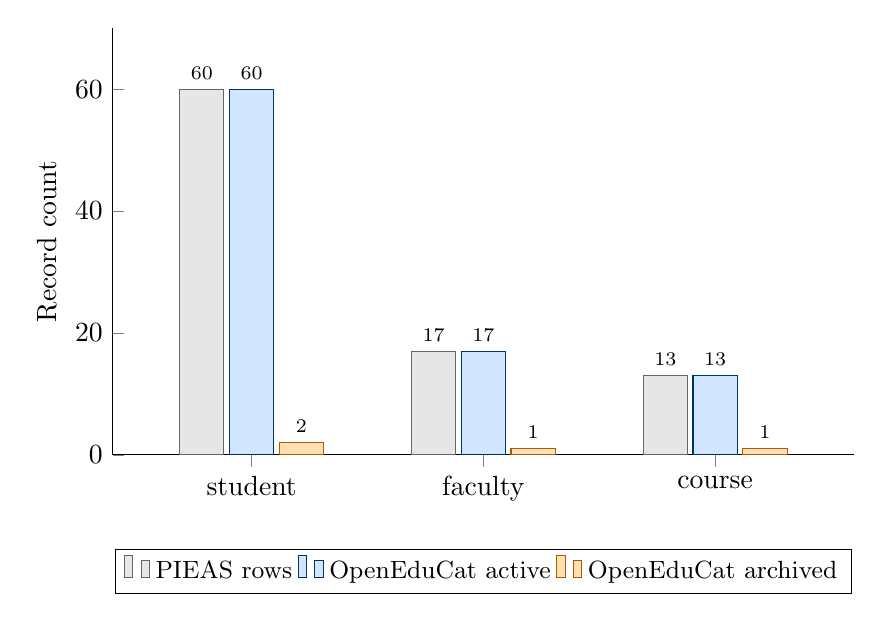
\begin{tikzpicture}
\begin{axis}[
    ybar,
    bar width=16pt,
    width=11cm, height=7cm,
    symbolic x coords={student,faculty,course},
    xtick=data,
    ylabel={Record count},
    ymin=0, ymax=70,
    legend style={at={(0.5,-0.22)}, anchor=north, legend columns=-1, font=\small},
    nodes near coords,
    every node near coord/.append style={font=\scriptsize},
    enlarge x limits=0.3,
    axis lines*=left,
]
\addplot[fill=StoreGray, draw=black!60] coordinates {(student,60) (faculty,17) (course,13)};
\addplot[fill=AgentBlue, draw=NavyBlue] coordinates {(student,60) (faculty,17) (course,13)};
\addplot[fill=OrchOrange, draw=orange!70!black] coordinates {(student,2) (faculty,1) (course,1)};
\legend{PIEAS rows, OpenEduCat active, OpenEduCat archived}
\end{axis}
\end{tikzpicture}
\caption{PIEAS row counts vs.\ OpenEduCat active/archived counts per entity type, after the full
demo lifecycle. PIEAS row counts equal OpenEduCat active counts in every case -- the sync stayed
consistent end to end.}
\label{fig:entitychart}
\end{figure}

% =========================================================================
\section{Known Characteristics and Limitations}
% =========================================================================

\begin{itemize}[leftmargin=1.4em]
    \item \textbf{Re-archiving a permanently-deleted record.} Discussed in
          Section~\ref{sec:change-deletion} -- harmless, but worth knowing about when reading
          deletion-cycle reports.
    \item \textbf{No LLM in the loop.} The Transformer's field mapping is deterministic
          Python, not an LLM call. This was a deliberate choice for a synchronization pipeline
          that must be exactly reproducible and fully unit-testable; an LLM-assisted mapping
          step could be added later for messier real-world source schemas without changing any
          other agent.
    \item \textbf{Mock domain filtering.} \texttt{OpenEduCatClient.search\_read} supports only a
          flat AND of equality conditions -- enough for this pipeline's needs, not a general
          Odoo domain evaluator. A real XML-RPC connection supports Odoo's full domain
          language; this only matters if the mock client's surface is extended further.
    \item \textbf{Dummy data, not production data.} PIEAS record volumes, department names, and
          identifiers are illustrative (drawn from PIEAS's real academic departments for
          realism) but entirely synthetic.
\end{itemize}

% =========================================================================
\section{Path to Production}
% =========================================================================

The system was deliberately built so that pointing it at the real PIEAS database and a real
self-hosted Odoo + OpenEduCat instance touches exactly \textbf{two files}:

\begin{table}[H]
\centering
\small
\begin{tabular}{@{}p{3.6cm}p{10.4cm}@{}}
\toprule
\textbf{File to change} & \textbf{What changes} \\
\midrule
\texttt{pieas\_source.py} & Replace the SQLite connection with whatever PIEAS's real database
is (or a read-only integration layer), exposing the same \texttt{fetch\_changed} /
\texttt{fetch\_page} / \texttt{fetch\_ids} function shapes. \texttt{ExtractorAgent} does not
change. \\
\texttt{openeducat\_client.py} & Replace the SQLite-backed methods with real
\texttt{xmlrpc.client.ServerProxy} calls against Odoo's \texttt{common}/\texttt{object}
endpoints (\texttt{execute\_kw(db, uid, password, model, method, args)}), keeping the same
\texttt{create}/\texttt{write}/\texttt{archive}/\texttt{search\_read}/\texttt{read} method
signatures. \texttt{LoaderAgent} and \texttt{ValidationAgent} do not change. \\
\bottomrule
\end{tabular}
\caption{The entire production-swap surface.}
\end{table}

Everything else -- the Orchestrator's decision logic, the Transformer's field mappings, the
LangGraph wiring, the CLI, and the test suite's structure -- carries over unchanged, because the
whole system was built against the report's \emph{agent boundaries} rather than against SQLite
specifically.

% =========================================================================
\section{Conclusion}
% =========================================================================

The source report set out to design, not build, an agentic multi-agent system solving two
coupled problems: a one-time bulk migration and an ongoing, agentic synchronization (including
deletion handling) between a source system with no API and a target ERP with a well-documented
ORM. This project completes that design into working, tested software: four agents with
strictly non-overlapping responsibilities, wired as a single LangGraph state machine that serves
all three of the report's cycles, running against reproducible dummy data through database
boundaries that make the report's ownership rules impossible to violate by accident -- verified
by 57 passing tests and a one-command, end-to-end demo.

\appendix
% =========================================================================
\section{Appendix: Project File Tree}
% =========================================================================

\begin{lstlisting}[style=termstyle,basicstyle=\ttfamily\scriptsize\color{white}]
src/openedu_orchestrator/
    config.py              # DB paths, entity types, schedule constants
    models.py               # pydantic schemas (PieasStudent/Faculty/Course, RunReport, ...)
    state.py                 # LangGraph PipelineState TypedDict
    pieas_source.py          # dummy PIEAS DB (schema, seeding/mutation/read helpers)
    openeducat_client.py     # mock Odoo/OpenEduCat ORM-shaped client
    sync_store.py            # sync_mapping / sync_state -- Orchestrator-only
    seed.py                  # deterministic Faker-based dummy data generator
    graph.py                 # LangGraph StateGraph wiring + run_cycle()
    cli.py                   # click CLI
    agents/
        extractor.py
        transformer.py
        loader.py
        orchestrator.py
        validator.py
tests/                       # pytest suite (57 tests)
\end{lstlisting}

\end{document}
